                            \documentclass{article}
\documentclass{article}
\usepackage[utf8]{inputenc}
\usepackage[table]{xcolor}
\usepackage{graphicx}
\usepackage[T1]{fontenc}
\usepackage{imakeidx}
\usepackage{imakeidx}
\usepackage{tabularx}
\usepackage{booktabs}
\usepackage{outlines}
\usepackage{forloop}
\usepackage{pgfgantt}
\usepackage{comment}
\usepackage{xcolor,colortbl}
\usepackage[export]{adjustbox}
\makeindex[name=Alphabetical,title={Alphabetical Index},columns=1]
\makeindex[name=Models,title={Index of Models},columns=1]

\newcounter{loopcntr}
\newcommand{\rpt}[2][1]{%
  \forloop{loopcntr}{0}{\value{loopcntr}<#1}{#2}%
}
\newcommand{\on}[1][1]{
  \forloop{loopcntr}{0}{\value{loopcntr}<#1}{&\cellcolor{gray}}
}
\newcommand{\off}[1][1]{
  \forloop{loopcntr}{0}{\value{loopcntr}<#1}{&}
}


\title{Architecture and Design document} % Sets article title
\author{Artin Ghalamkary - (AU677595) \and Karsten Bak Malle - (AU644054) \and Nikita Svanholm Alsøer - (AU639436) \and Phillip Ravn Boe Jensen - (AU681033)}% Sets authors name
\date{15-10-2021}

\begin{document}




\maketitle
\section*{Preface} \index[Alphabetical]{Preface}
The architecture and design document include documentation which describe components and specifications of the mail client. The document may not contain every or describe every component or specification of the mail client, because there may be changes in future based on different factor which could impact the design of the mail client. However it is expected that other components may be added in the future, presumably with more in-depth description and more detailed diagrams.


\section*{Introduction} \index[Alphabetical]{Introduction}
The purpose of this document is to ensure that the user has a solid understanding of the mail client. The goal is to graphically and descriptively clarify the components as well as the relations involved in our system architecture.

\newpage

\section*{Glossary} \index[Alphabetical]{Glossary}
\begin{enumerate} 
    \item \textbf{Stakeholder:}\index[Alphabetical]{Stakeholder} refers to individuals, groups or organizations that have any type of relation or interest in the development of the software product.
    \item \textbf{Python:}\index[Alphabetical]{Python} is a computer programming language often used to build websites and software, automate tasks and analyse data. 
    \item \textbf{Web framework:}\index[Alphabetical]{Web framework} is a tool/resource designed to support the development of web applications.
    \item \textbf{Django:}\index[Alphabetical]{Django} is a Python based web framework that enables fast, secure and maintainable web applications. 
    \item \textbf{Front-end:}\index[Alphabetical]{Front-end} is the part of the application which the customer is able to interact with, this can be such as the graphical user interface, or navigation between menus.
    \item \textbf{Middleware:}\index[Alphabetical]{Middleware} as the name suggest is the software which lies between the application and the operating system they use.
    \item \textbf{Backend:}\index[Alphabetical]{Backend} is the part of the software which the customer will not see, for example that could be the database where certain data is stored or maybe a website request. 
\end{enumerate}

\newpage

\section*{Architectural Representation}\index[Alphabetical]{Architectural Representation}

The architectural representation here describes how the system implements the software architecture. The goal here is to graphically represent the important decisions that are taken, as well as the structural elements and how the components are connected.

\subsection*{Use Case}\index[Alphabetical]{Use Case}
To represent the architecture of our system, we have chosen to implement the Use-Case Modeling, which, as short described above, has the goal of graphically showing the actors, in our case the user and recipients, as well as the relationships between them.

\subsection*{Association diagram}\index[Alphabetical]{Association diagram}
The following diagram demonstrates the association between the user and email addresses. The diagram states that the user is allowed to use more than one email address, when using the email client. 

\begin{center}
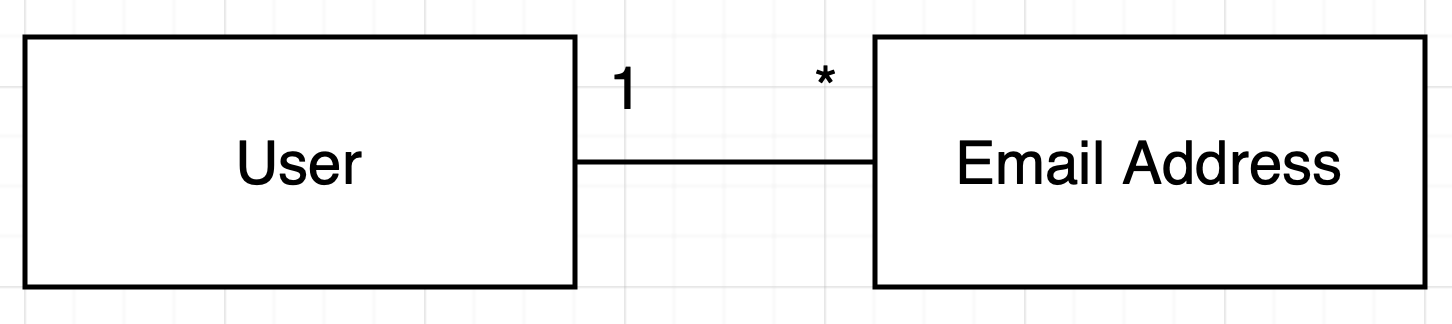
\includegraphics[width=350px, keepaspectratio]{UML_Association..png}\\[1cm]\index[Alphabetical]{Association diagram} \index[Models]{Association diagram}
\end{center} 

\newpage

\subsection*{Class diagram}\index[Alphabetical]{Class diagram}
The diagram beneath is the Email class diagram, which is a general diagram with the different methods, that defines the functionality of the mail client. We use generalization to make it easier for us to handle changes, which makes it easier to manage the complexity of the email client. 
\vspace{6 mm}

\begin{center}
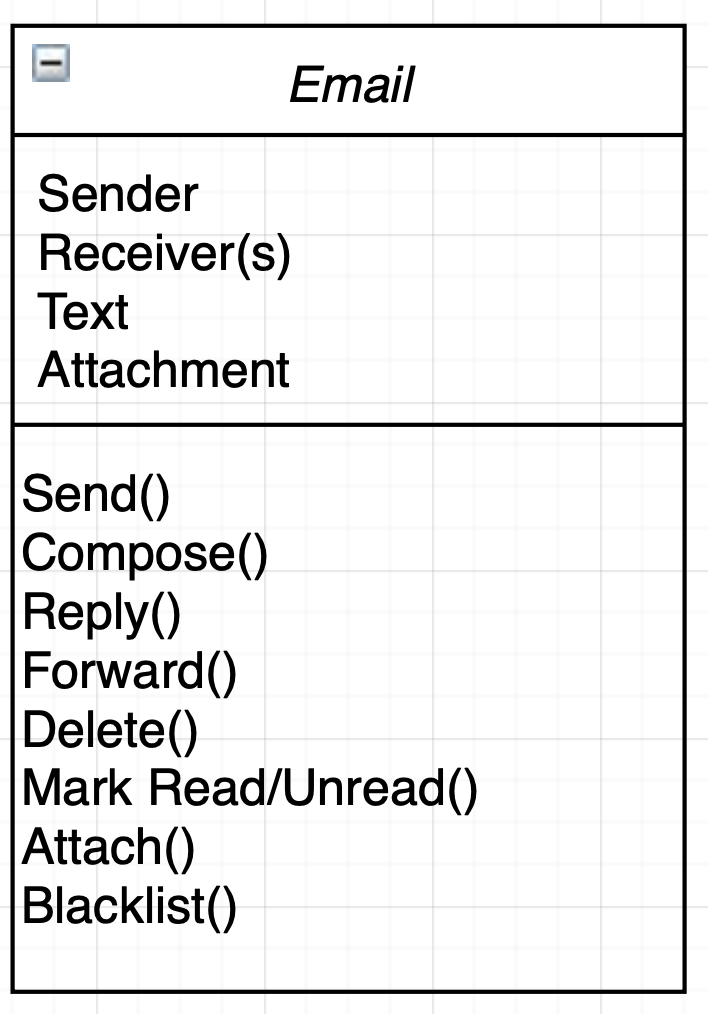
\includegraphics[width=200px, keepaspectratio]{Class_Diagram.png}\\[1cm]\index[Models]{Class diagram}
\end{center}

\newpage

\section*{Architectural Goals and Constraints}
\begin{flushleft}
\textbf{Architectural Goals:}\\ \index[Alphabetical]{Architectural Goals}

\end{flushleft}
\begin{outline}
    \1 Meet the requirements of the stakeholder.  
    \1 Display the structure of the system.
    \1 Recognize all the use-cases.
    \1 Protect and secure sensitive information. 
\end{outline}
\begin{flushleft}
\textbf{Architectural Constraints:}\\ \index[Alphabetical]{Architectural Constraints}

\end{flushleft}
\begin{outline}
    \1 Follow the schedule to deliver on time.
    \1 By choosing Python we created a constraint on ourselves. We are restricted to Python specific frameworks.
\end{outline}

\newpage

\section*{Use-case Model}\index[Alphabetical]{Use-case Model}


\begin{figure}[h]
  \noindent\makebox[\textwidth]{%
  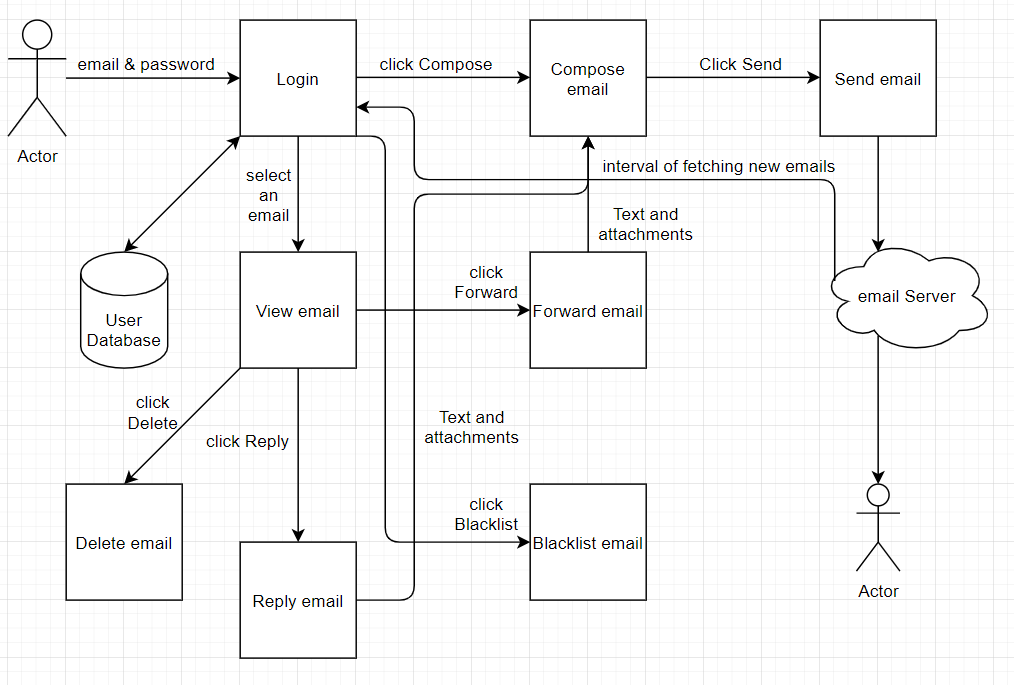
\includegraphics[width=1.4\textwidth]{Dataflowchart.png}}
\end{figure} \index[Models]{Use-case}


\newpage

\section*{Use-case explained in detail} \index[Models]{Use-case explained}
\renewcommand{\labelenumii}{\arabic{enumi}.\arabic{enumii}}
\begin{enumerate} 
    \item \textbf{Login:} If the user has completed the \textit{Login} stage before then this stage is skipped since the \textit{User Database} already has the user's information stored. If the user has \textbf{NOT} completed the \textit{Login} stage then user will need to provide an email and password to continue.
    \item \textbf{Inbox:} Our inbox updates in intervals, using the email server linked with the users email address. After \textit{Login} we have a overview of our inbox containing all our emails, this gives us $4$ options.
    \begin{enumerate}
        \item \textbf{View email:} If we choose to view our email we can either \textit{Delete email}, \textit{Reply email} or \textit{Forward email}. \textit{Delete email} will delete the email we are viewing. \textit{Reply email} takes the sender address of the email we are viewing and composes a new email with that address as the destination. \textit{Forward email} will copy the text and attachment(s) of the email we are viewing and compose a new email with the copied text and attachment(s). 
        \item \textbf{Compose email:} Will either be an extension of \textit{Forward email} / \textit{Reply email} or simply create a new blank email. When the user is done editing the desired email it can then be sent by clicking the send button \textit{Send email} to the receiver.
        \begin{itemize}
            \item \textbf{Send email:} is an extension of \textit{Compose email}. By using the email address of the receiver, we connect with the email server linked with the recipients email address which then fetches our email. 
        \end{itemize}
        \item \textbf{Blacklist email:} If chosen, the user is able to \textit{Blacklist} any mail of choosing, which will sort the blacklisted emails in a separate folder different from the main \textit{Inbox}. The user can at any time remove a given email address from the \textit{Blacklist}.
        \item \textbf{Logout:} takes us back to the \textit{Login} stage. This means we have to go through the \textit{Login} stage once again to get to our \textit{Inbox}.
    \end{enumerate}
    
\end{enumerate}

\newpage

\section*{Architectural Pattern}\index[Alphabetical]{Architectural Patterns}

\subsection*{Model-Template-View with Django}\index[Alphabetical]{Pattern: Model-Template-View}\index[Alphabetical]{Django}

The email client is being  developed using a python-based web-framework called Django. Django follows models-template-view (mtv) architectural pattern. Using such an architectural pattern will provide us with a basis for our email client. The diagram below how the Django web-frame works using the mtv model. Looking at the diagram it is possible to see that the work load is split into different levels, the client side, the server side and database. At the client side level, the front-end work happens such as designing the graphical view of the mail client, while at the server side consists of the middleware and backend. 
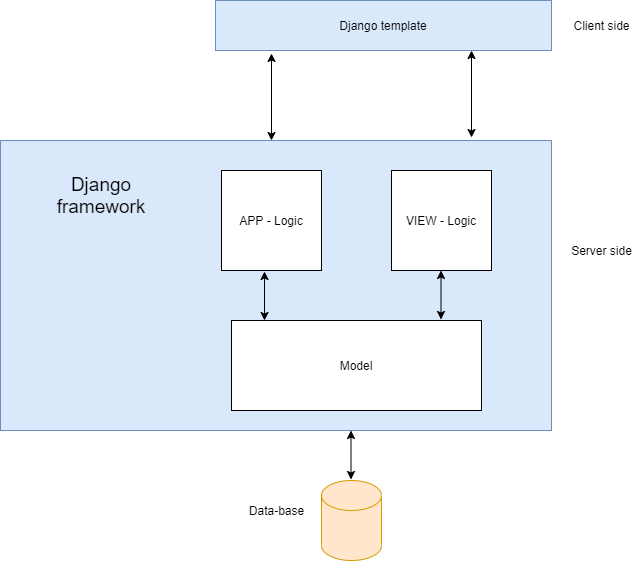
\includegraphics[width=300px, keepaspectratio]{Django.png}\\[1cm]
\vspace{-15 mm}


\newpage

\section*{Responsibilities}\index[Alphabetical]{Responsibilities}\index[Alphabetical]{Responsibilities}
Using Django to develop the mail client, it have made it easy to divide the roles between the company employees, because there is a clear view of what is front-end, middle-end and backend and how it can be tackled using Django. \\

The responsibilities looks as follows:
\begin{enumerate}
    \item 1 Front-end developer
    \item 2 Middleware developers
    \item 1 Backend developer
\end{enumerate}

\newpage


\printindex[Alphabetical]
\printindex[Models]

\end{document}

